\section{Resultados con materiales reales: Au y Ag}
\label{section:AuAg}

Con la finalidad de presentar la respuesta óptica de una monocapa de NPs conformadas por materiales realista, se emplea en esta sección la función dieléctrica con corrección por tamaño para NPs esféricas de oro [Fig. \ref{sfig:sizeAu}] y de plata [Fig. \ref{sfig:sizeAg}]. La elección de NPs de oro y plata surge a partir de su uso en el biosensado \cite{jain2008noble}, así como por su biocompatibilidad \cite{fan2009bio,bosetti2002silver}. Los cálculos realizados corresponden a la reflectancia y transmitancia en configuración ATR, puesto que en el análisis con las funciones dieléctrica tipo Drude fue en donde se observó la presencia de un modo distinto a las excitaciones de partículas individuales. Asimismo, se realizó el análisis de la transmitancia para corroborar que las excitaciones presentes para materiales realistas presentan un comportamiento semejante al modo guiado reportado en \cite{kabashin2009plasmonic} y \cite{danilov2018ultra}, también observado en sistemas de NPs desordenadas con una función dieléctrica tipo Drude.

En la Fig.  \ref{fig:Au-R-Theta} se muestran los cálculos de la reflectancia $R$, empleando el CSM, de una monocapa de NPs esféricas idénticas de oro con un radio de $a = 30$ nm, inmersa en una matriz de aire ($n_m = 1$) y soportada por un sustrato con un índice de refracción $n_s = 1.5$, que es iluminada por una onda plana en una configuración ATR. La reflectancia se grafica como función del ángulo de incidencia $\theta_i$ y tanto de la longitud de onda $\lambda$ (escala inferior), así como de la energía en unidades de $\hbar\omega$ (escala superior). Se consideraron las fracciones de cubierta $\Theta = 0.05,\,0.1,\,0.2,\,0.3$, así como la polarización de la onda plana incidente: las gráficas \textbf{i)}--\textbf{iv)} corresponden a la polarización \emph{p} y \textbf{v)}--\textbf{viii)} a \emph{s}. Las líneas punteadas verticales verdes y rosas corresponden a las SP-SPRs dipolares y cuadrupolares, respectivamente: para el una NP de oro de $a= 30$ nm la SP-SPR dipolar se localiza en $\lambda = 512$ nm y la cuadrupolar en $498$ nm, como se observa en la Fig. \ref{fig:Au-R-Theta}.

	\begin{figure}[h!]\centering
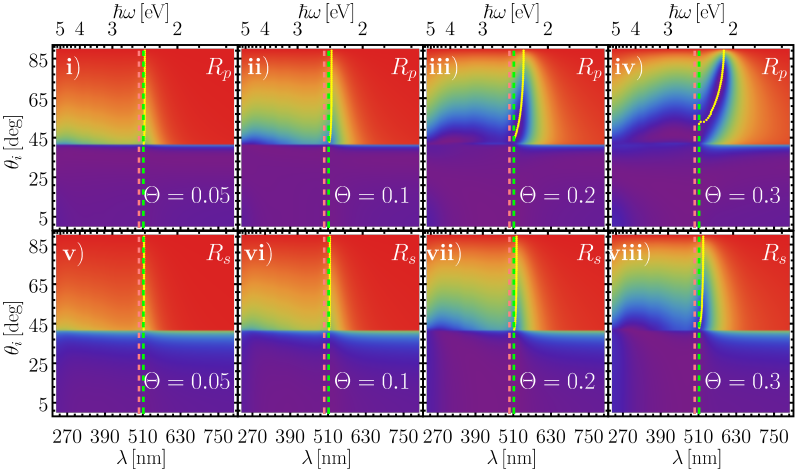
\includegraphics[width = .75\linewidth]{2-Resultados/figs/6-AuThetaVar/0-2D_Grid}%
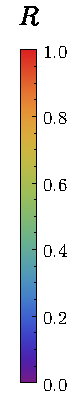
\includegraphics[scale=.85, trim={00 -5 00 00}, clip]{2-Resultados/figs/0-RBar_v}
	\caption{Gráficas de reflectancia de una monocapa de NPs esféricas de oro de radio $a=30$ nm en configuración ATR como función del ángulo de incidencia $\theta_i$ y de la longitud de onda $\lambda$ (escala inferior), así como de la energía del haz incidente en unidades de $\hbar\omega$ (escala superior).  Las gráficas   en el renglón superior [$\mathbf{i)-v)}$] muestran los resultados para  polarización \emph{p} y las del renglón inferior  [$\mathbf{vi)-x)}$]  para polarización  \emph{s}, donde se consideraron los valores de fracción de cubierta $\Theta = 0.05,\,0.1,\,0.2$ y $0.3$.  Las líneas verticales punteadas verdes y rosas corresponden a las SP-SPRs dipolar en $\lambda=512$ nm y  cuadrupolar en $\lambda=498$, respectivamente.  Los puntos amarillos corresponden a los mínimos en $R$ para ángulos mayores a $\theta_c\approx 41^\circ$ y longitudes de onda mayores a la SP-SPRs dipolar.
}	\label{fig:Au-R-Theta}	
	\end{figure}	

A diferencia de los cálculos de la reflectacia de una monocapa de NPs  con una función dieléctrica tipo Drude analizada en la sección \ref{ssection:DrudeATR}, en donde sólo se presentaron excitaciones al rededor de las SP-SPRs y el modo colectivo a longitudes de onda mayores a las de las SP-SPRs, los cálculos de la monocapa de NPs de de oro muestran excitaciones a valores de $\lambda$ menores a las de las SP-SPRs (líneas verticales punteadas), las cuales corresponden a excitaciones no plasmónicas, es decir, a contribuciones de transiciones de electrones ligados. Sin embargo, dado que el modo colectivo se excita a energías menores a las de las transiciones interbanda, su contribución no afecta a la excitación colectiva y ésta aún es apreciable, como se observa en las gráficas \textbf{iii), iv), vii)} y \textbf{viii)} de la Fig. \ref{fig:Au-R-Theta}. El modo colectivo, es apreciable para las fracciones de cubierta empleadas de mayor valor ($\Theta = 0.2, 0.3$) y, como sucedió para el análisis con una función dieléctrica tipo Drude, el modo colectivo se aprecia más para polarización \emph{p}, además de traslaparse con la SP-SPRs dipolar.

La reflectancia de una monocapa de NPs con las mismas características que las de la Fig. \ref{fig:Au-R-Theta} pero con NP esféricas de plata de radio $a=30$ nm, se grafica en la Fig. \ref{fig:Ag-R-Theta}, en donde la SP-SPR dipolar corresponde a la línea vertical verde en $\lambda=368$ nm y la cuadrupolar, a la líneas vertical rosa en $\lambda=348$ nm. Al igual que para la monocapa de NPs de oro, se aprecian excitaciones no plasmónicas en valores de $\lambda$ menores a la de las SP-SPRs sin embargo, para la plata estas excitaciones están separadass de las plasmónicas, como se observa por la presencia de la región roja, al rededor de los $300$ nm,  en donde $R\approx 1$. De la misma forma, es apreciable en las gráficas de la Fig. \ref{fig:Ag-R-Theta} el modo colectivo que, para algunos casos, también se separa de la SP-SPRs permitiendo observar ambas.

\begin{figure}[h!]\centering
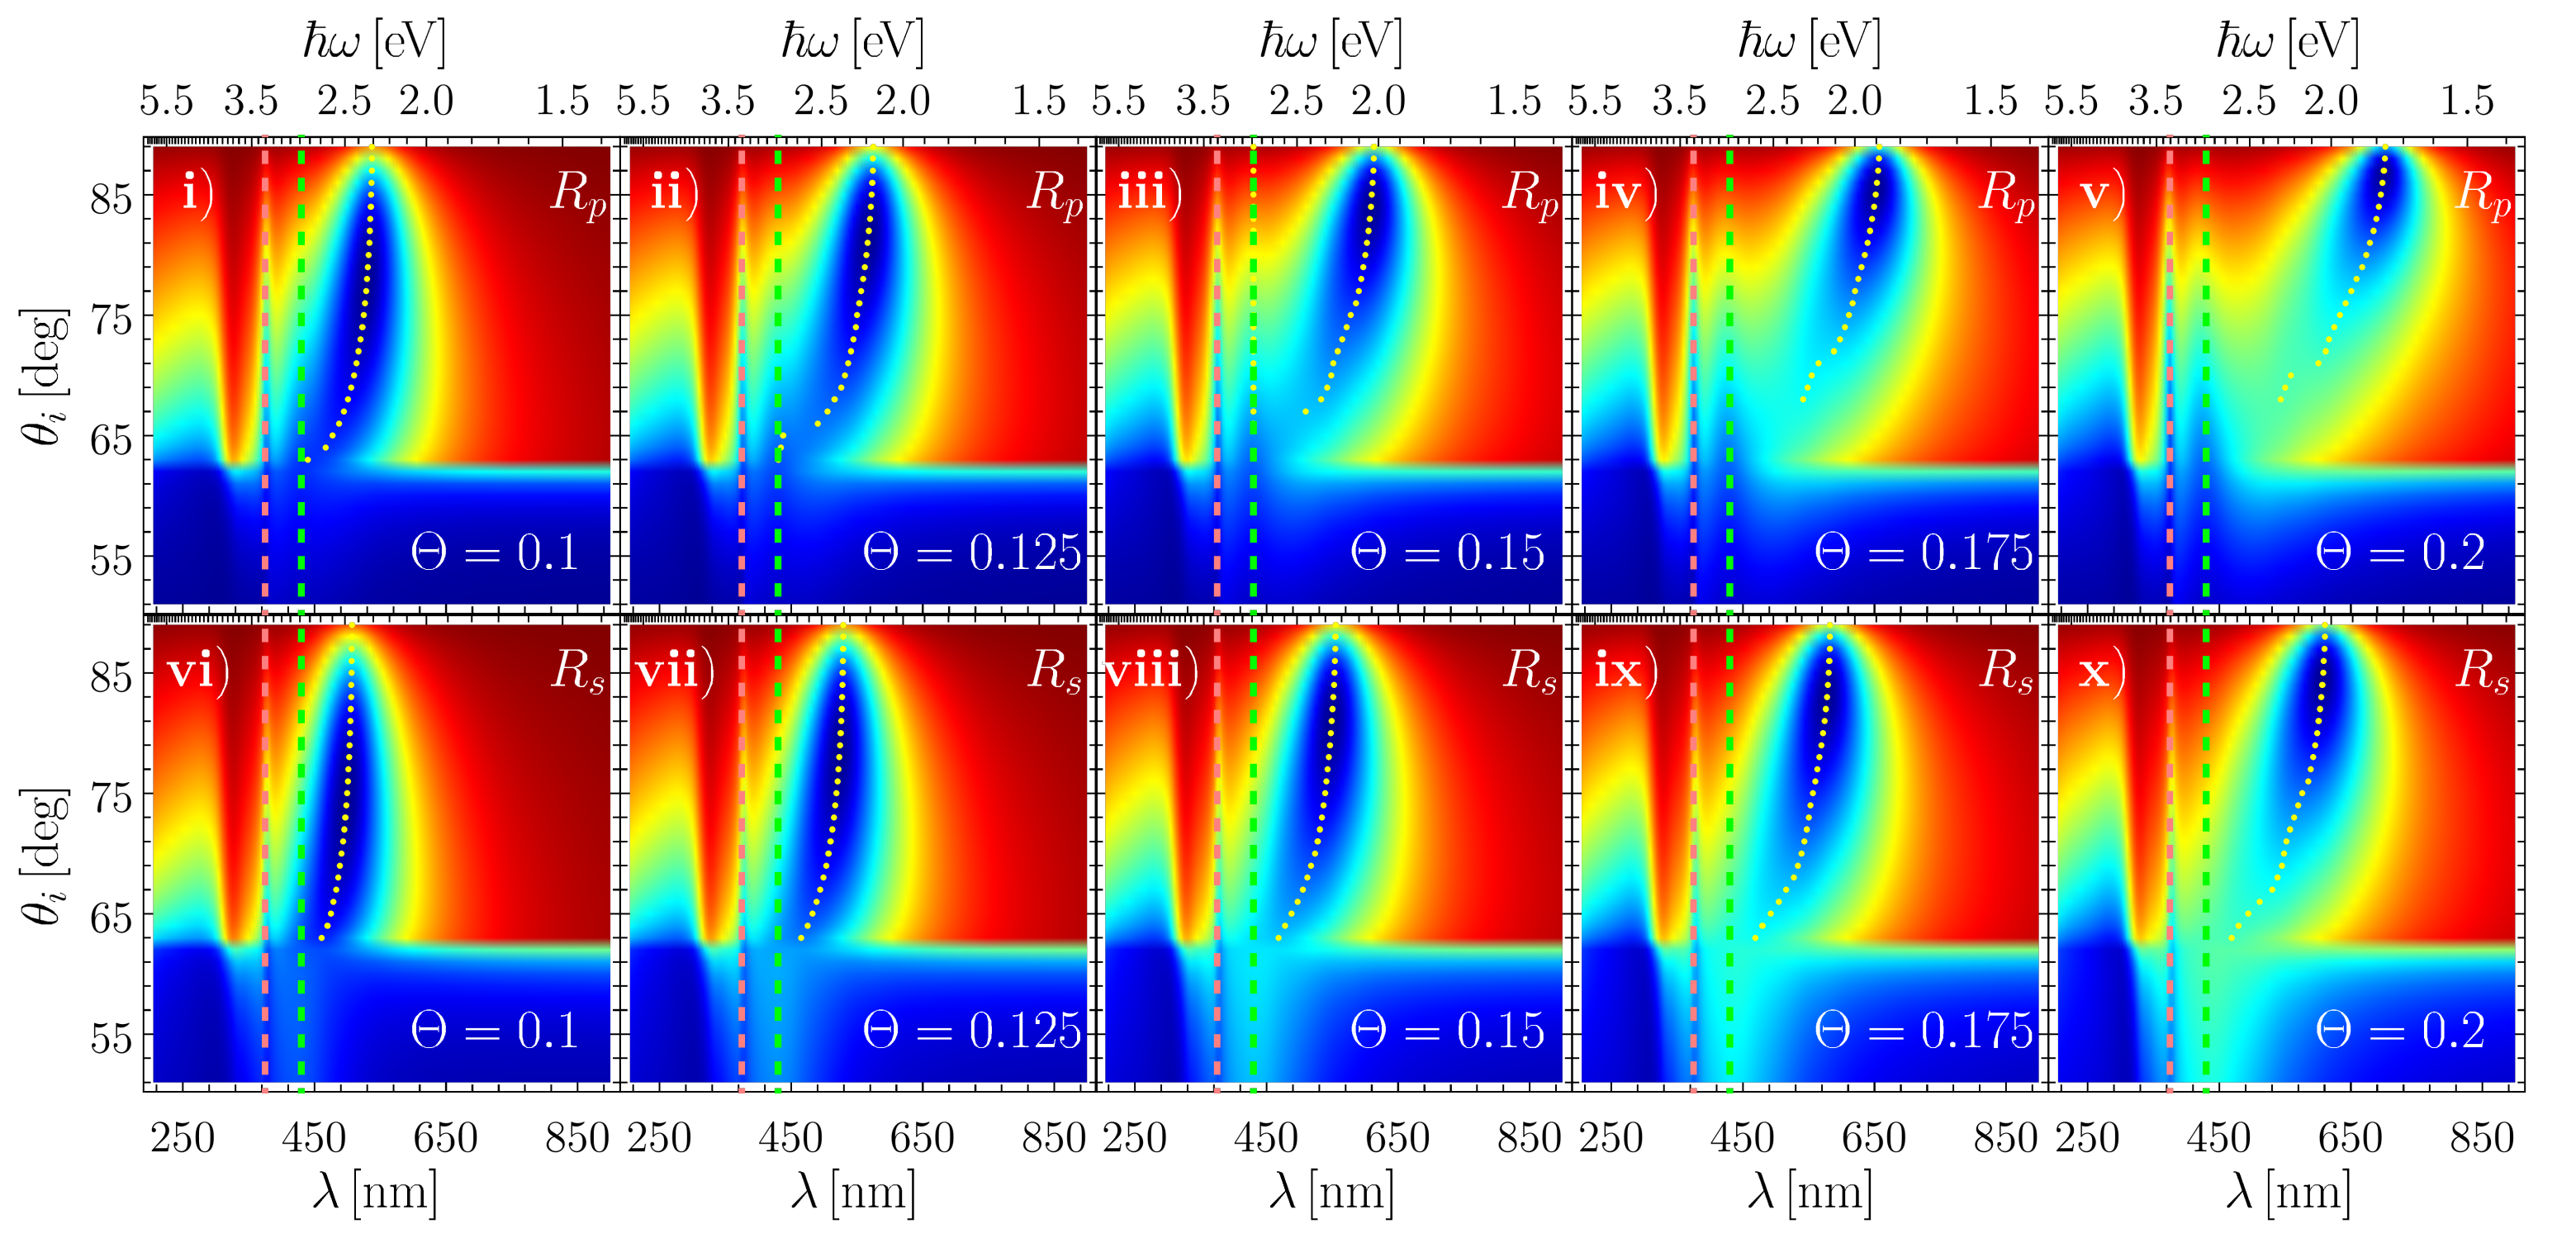
\includegraphics[width = .75\linewidth]{2-Resultados/figs/7-AgThetaVar/0-2D_Grid}%
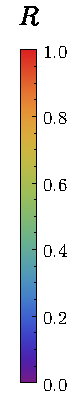
\includegraphics[scale=.85, trim={00 -5 00 00}, clip]{2-Resultados/figs/0-RBar_v}
	\caption{Gráficas de reflectancia de una monocapa de NPs esféricas de plata de radio $a=30$ nm en configuración ATR como función del ángulo de incidencia $\theta_i$ y de la longitud de onda $\lambda$ (escala inferior), así como de la energía del haz incidente en unidades de $\hbar\omega$ (escala superior).  Las gráficas   en el renglón superior [$\mathbf{i)-v)}$] muestran los resultados para  polarización \emph{p} y las del renglón inferior  [$\mathbf{vi)-x)}$]  para polarización  \emph{s}, donde se consideraron los valores de fracción de cubierta $\Theta = 0.05,\,0.1,\,0.2$ y $0.3$.  Las líneas verticales punteadas verdes y rosas corresponden a las SP-SPRs dipolar en $\lambda=368$ nm y  cuadrupolar en $\lambda=348$, respectivamente.  Los puntos amarillos corresponden a los mínimos en $R$ para ángulos mayores a $\theta_c\approx 41^\circ$ y longitudes de onda mayores a la SP-SPRs dipolar.
}	\label{fig:Ag-R-Theta}	
	\end{figure}	

El modo colectivo, al igual que con la monocapa de NPS de oro, es apreciable al emplear plata, como se observa en las gráficas \textbf{ii) -- iv), vii)} y \textbf{viii)}, siendo la polarización \emph{p} (gráficas del renglón superior de la Fig. \ref{fig:Ag-R-Theta}) en donde el modo colectivo es más apreciable. Igualmente, las SP-SPRs se distinguen de la excitación colectiva para los valores de $\Theta\geq 0.1$  para polarización \emph{p}, mientras que para polarización \emph{s} las excitaciones de partícula individual se traslapan con el modo colectivo para todos los casos de $\Theta=0.2$ y $0.3$. Para $\Theta = 0.05$ y $0.1$ y polarización \emph{s}, el modo colectivo no es apreciable, como tampoco lo es para $\Theta=0.05$ en polarización \emph{p}.

Dado que el modo colectivo se presenta para monocapas de NPs tanto de oro como de plata, ambos materiales pueden emplearse en el biosensado. Para analizar las diferencias entre la respuesta EM de una monocapa de NPs esféricas de oro y plata, se grafican, en la Fig. \ref{fig:AuAg-Cuts}, cortes a $\theta_i = 65^\circ$ de la reflectancia de la Fig. \ref{fig:Au-R-Theta}, donde se emplean NPs de oro, y de la Fig. \ref{fig:Ag-R-Theta}, donde se consideran NPs de plata. En las Figs. \ref{sfig:Au-cutp} y \ref{sfig:Au-cuts} se grafica la reflectancia para una monocapa de NPs de oro al incidir una onda plana con polarización \emph{p} y \emph{s}, respectivamente, mientras que en las Figs. \ref{sfig:Ag-cutp} y \ref{sfig:Ag-cuts} se grafica la reflectancia para una monocapa de NPs de plata para polarización \emph{p} y \emph{s}, respectivamente.

\begin{figure}[h!]\centering\hspace*{-1.5em}
	\begin{subfigure}{.01\linewidth}\caption{}\label{sfig:Au-cutp}\vspace{4.5cm}\end{subfigure}
	\begin{subfigure}{.45\linewidth}\hspace*{-1.5em}
	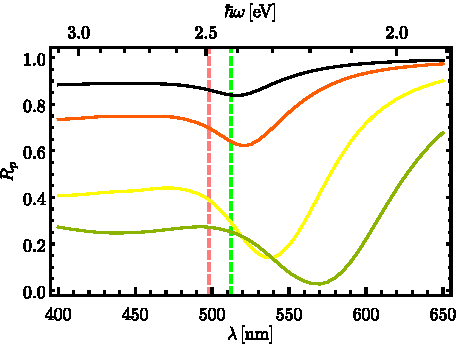
\includegraphics[scale=1]{2-Resultados/figs/6-AuThetaVar/cut_angle_65_p.pdf}\end{subfigure}
	\begin{subfigure}{.01\linewidth}\caption{}\label{sfig:Au-cuts}\vspace{4.5cm}\end{subfigure}\hspace*{-1.em}
	\begin{subfigure}{.45\linewidth}\centering
	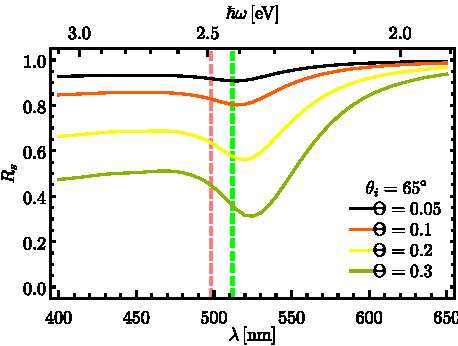
\includegraphics[scale=1 ]{2-Resultados/figs/6-AuThetaVar/cut_angle_65_s.pdf}\end{subfigure}\vspace*{0em}\\
	\hspace*{-1.5em}
	\begin{subfigure}{.01\linewidth}\caption{}\label{sfig:Ag-cutp}\vspace{4.5cm}\end{subfigure}
	\begin{subfigure}{.45\linewidth}\hspace*{-1.5em}
	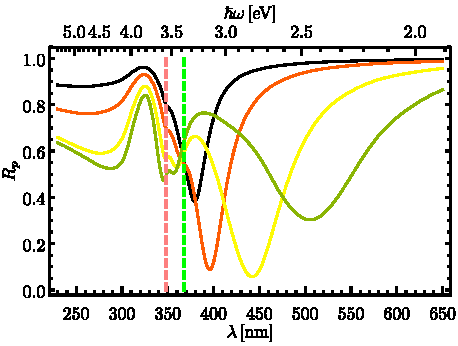
\includegraphics[scale=1]{2-Resultados/figs/7-AgThetaVar/cut_angle_65_p.pdf}\end{subfigure}
	\begin{subfigure}{.01\linewidth}\caption{}\label{sfig:Ag-cuts}\vspace{4.5cm}\end{subfigure}\hspace*{-1.em}
	\begin{subfigure}{.45\linewidth}\centering
	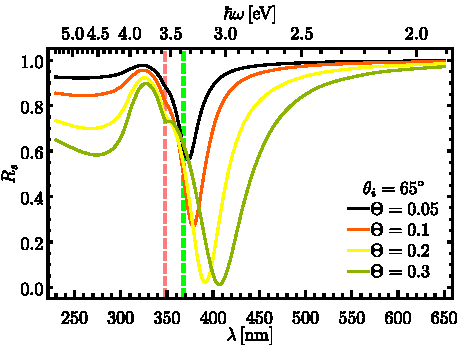
\includegraphics[scale=1 ]{2-Resultados/figs/7-AgThetaVar/cut_angle_65_s.pdf}\end{subfigure}\vspace*{-.7em}
	\caption{Cortes a $\theta_i = 65^\circ$ de las gráficas de reflectancia de una monocapa en configuración ATR (Fig. \ref{fig:R-RVar}) de NPs esféricas de fracción de cubierta $\Theta = 0.3$ en polarización \textbf{a)} \emph{p} y \textbf{b)} \emph{s} como función de la longitud de onda $\lambda$ (escala inferior) y de la energía $\hbar\omega$ (escala superior). Los parámetros de la función dieléctrica tipo Drude para las NPs son $\omega_p = 4.3$ eV y $\gamma = 0.15$ eV y las fracciones de cubierta consideradas fueron $a$: $3$ nm, $5$ nm, $10$ nm y $20$ nm. La SP-SPR dipolar para los tamaños de partículas utilizadas corresponde la región verde entre $500$ nm y $512$ nm, mientras que la cuadrupolar corresponde a la región rosa entre $456$ nm y $462$ nm.}\label{fig:AuAg-Cuts}
	\end{figure}	

Los resultados para la monocapa de NPs de oro de $a=30$ nm presentan una menor reflectancia en el intervalo de $500$ nm$<\lambda<650$ nm para ambas polarizaciones conforme aumenta la fracción de cubierta $\Theta$. Asimismo, se presenta sólo un mínimo en los cálculos de la reflectancia para ambas polarizaciones que se corre al rojo, además de ser más pronunciado, conforme aumenta el valor de $\Theta$. Como se observó en la Fig. \ref{fig:Au-R-Theta}, las SP-SPRs no son apreciables para ninguna polarización, excepto en el caso de $\Theta =0.05$, donde el efecto de partícula individual es válido y por tanto la SP-SPR dipolar coincide con la única excitación presente en $\lambda = 512$ nm. Al comparar las Figs. \ref{sfig:Au-cutp} y \ref{sfig:Au-cuts} se corrobora que el corrimiento al rojo de la única excitación apreciable  es mayor para polarización \emph{p}, al igual que el decrecimiento en la reflectancia, como se observa en el caso de $\Theta=0.2$, donde para polarización \emph{p} el mínimo en reflectancia se localiza a $\lambda\approx  540$ nm  y $R \approx 0.2$, mientras que en polarización \emph{s}, $\lambda\approx 520$ nm y $R\approx 0.5$.

Cuando se consideran NPs de plata de $a=30$ nm para la monocapa, se presenta un máximo en la reflectancia tanto para polarización \emph{p} [Fig. \ref{sfig:Ag-cutp}] como para \emph{s} [Fig. \ref{sfig:Ag-cuts}]  a $\lambda \approx 330$ nm, valor de la longitud de onda que separa las excitaciones no plasmónicas ($\lambda<330$ nm) de las plasmónicas. Dentro de las SP-SPRs apreciables en la reflectancia de la monocapa se encuentra la resonancia cuadrupolar a $\lambda = 348$ nm (línea vertical rosa) para todos valores de $\Theta$ analizados y para ambas polarizaciones. En la Fig. \ref{sfig:Ag-cutp}, se aprecia en el intervalo $348$ nm$<\lambda<368$ nm y para $\Theta\geq 0.1$ un mínimo en $R_p$ que se corre al azul a valores de $\Theta$ mayores, por lo que puede ser un corrimiento al azul de la SP-SPR dipolar dado que la distancia promedio entre las NPs disminuye. El caso de $\Theta =0.05$, en polarización \emph{p}, no presenta ningún mínimo en la reflectancia a valores de $\lambda$ entre los de las SP-SPRs dipolar y cuadrupolar mas presenta un mínimo a $\lambda\approx 380$ nm, es decir, a longitudes de onda mayores, en donde $R_p\approx 0.4$. Para los casos de $\Theta = 0.1$ y $0.2$, también se aprecia un mínimo a longitudes de onda mayores que la de la SP-SPR dipolar y éste se corre al rojo conforme aumenta el valor de la fracción de cubierta, al igual que disminuye el valor de $R$, por ejemplo, para  $\Theta = 0.2$ el mínimo en $R_p$ se presenta a $\lambda \approx 440$ nm y $R_p \approx 0.05$. Esta tendencia sólo no se presenta para el caso de $\Theta = 0.3$ donde el valor de la reflectancia evaluada a la longitud de onda de la excitación ($\lambda \approx 510$ nm) aumenta respecto al del caso de $\Theta = 0.02$. Al considerar la polarización \emph{s} [Fig. \ref{sfig:Ag-cuts}], se aprecia únicamente la excitación a valores de $\lambda$ mayores a la de la SP-SPRs dipolar y ésta se corre al rojo y disminuye el valor de la reflectancia en estas longitudes de onda al crecer el valor de $\Theta$.

La respuesta EM de la monocapa de NPs tanto de oro como de plata presentan el comportamiento del modo colectivo a longitudes de onda mayores a las de la SP-SPRs dipolar (línea vertical verde en la Fig. \ref{fig:AuAg-Cuts}) sin embargo las características de esta excitación son distintas para cada uno de los materiales. Si bien para ambos materiales la resonancia colectiva se corre al rojo conforme aumenta la fracción de cubierta, para el oro  y \ref{sfig:Au-cuts}] ésta se localiza en el intervalo $512$ nm$<\lambda<570$ nm en polarización \emph{p} [ver Fig. \ref{sfig:Au-cutp}] y  en polarización \emph{s} en el intervalo  $512$ nm$<\lambda<530$ nm, es decir, que se encuentran dentro del espectro visible. Por otro lado, para la monocapa de NPs de plata, el modo colectivo se localiza para $\Theta = 0.05$ y $0.1$ en el ultravioleta para ambas polarizaciones; al aumentar $\Theta$, el modo colectivo se presenta a longitudes de onda entre $440$ nm y $520$ nm para polarización \emph{p} [ver Fig. \ref{sfig:Ag-cutp}] y entre $380$ nm y $410$ nm para polarización \emph{s} [ver Fig. \ref{sfig:Ag-cuts}]. Adicional al intervalo donde ocurre el modo colectivo, el valor de la reflectancia a los longitudes de onda de la excitación, así como el ancho de banda del modo colectivo, son menores para la monocapa de NPs de plata que para la de NPs de oro, por ejemplo, para la plata la reflectancia en los valores de $\lambda$ del modo colectivo es menor a $0.6$ para todos los casos como se observa en las Figs. \ref{sfig:Ag-cutp} y \ref{sfig:Ag-cuts}, mientras que para el oro $R<0.6$ sólo para $\Theta\geq 0.2$ [ver Figs. \ref{sfig:Ag-cutp} y \ref{sfig:Ag-cuts}].



 A diferencia del oro, el modo colectivo 



























\begin{figure}[h!]\centering
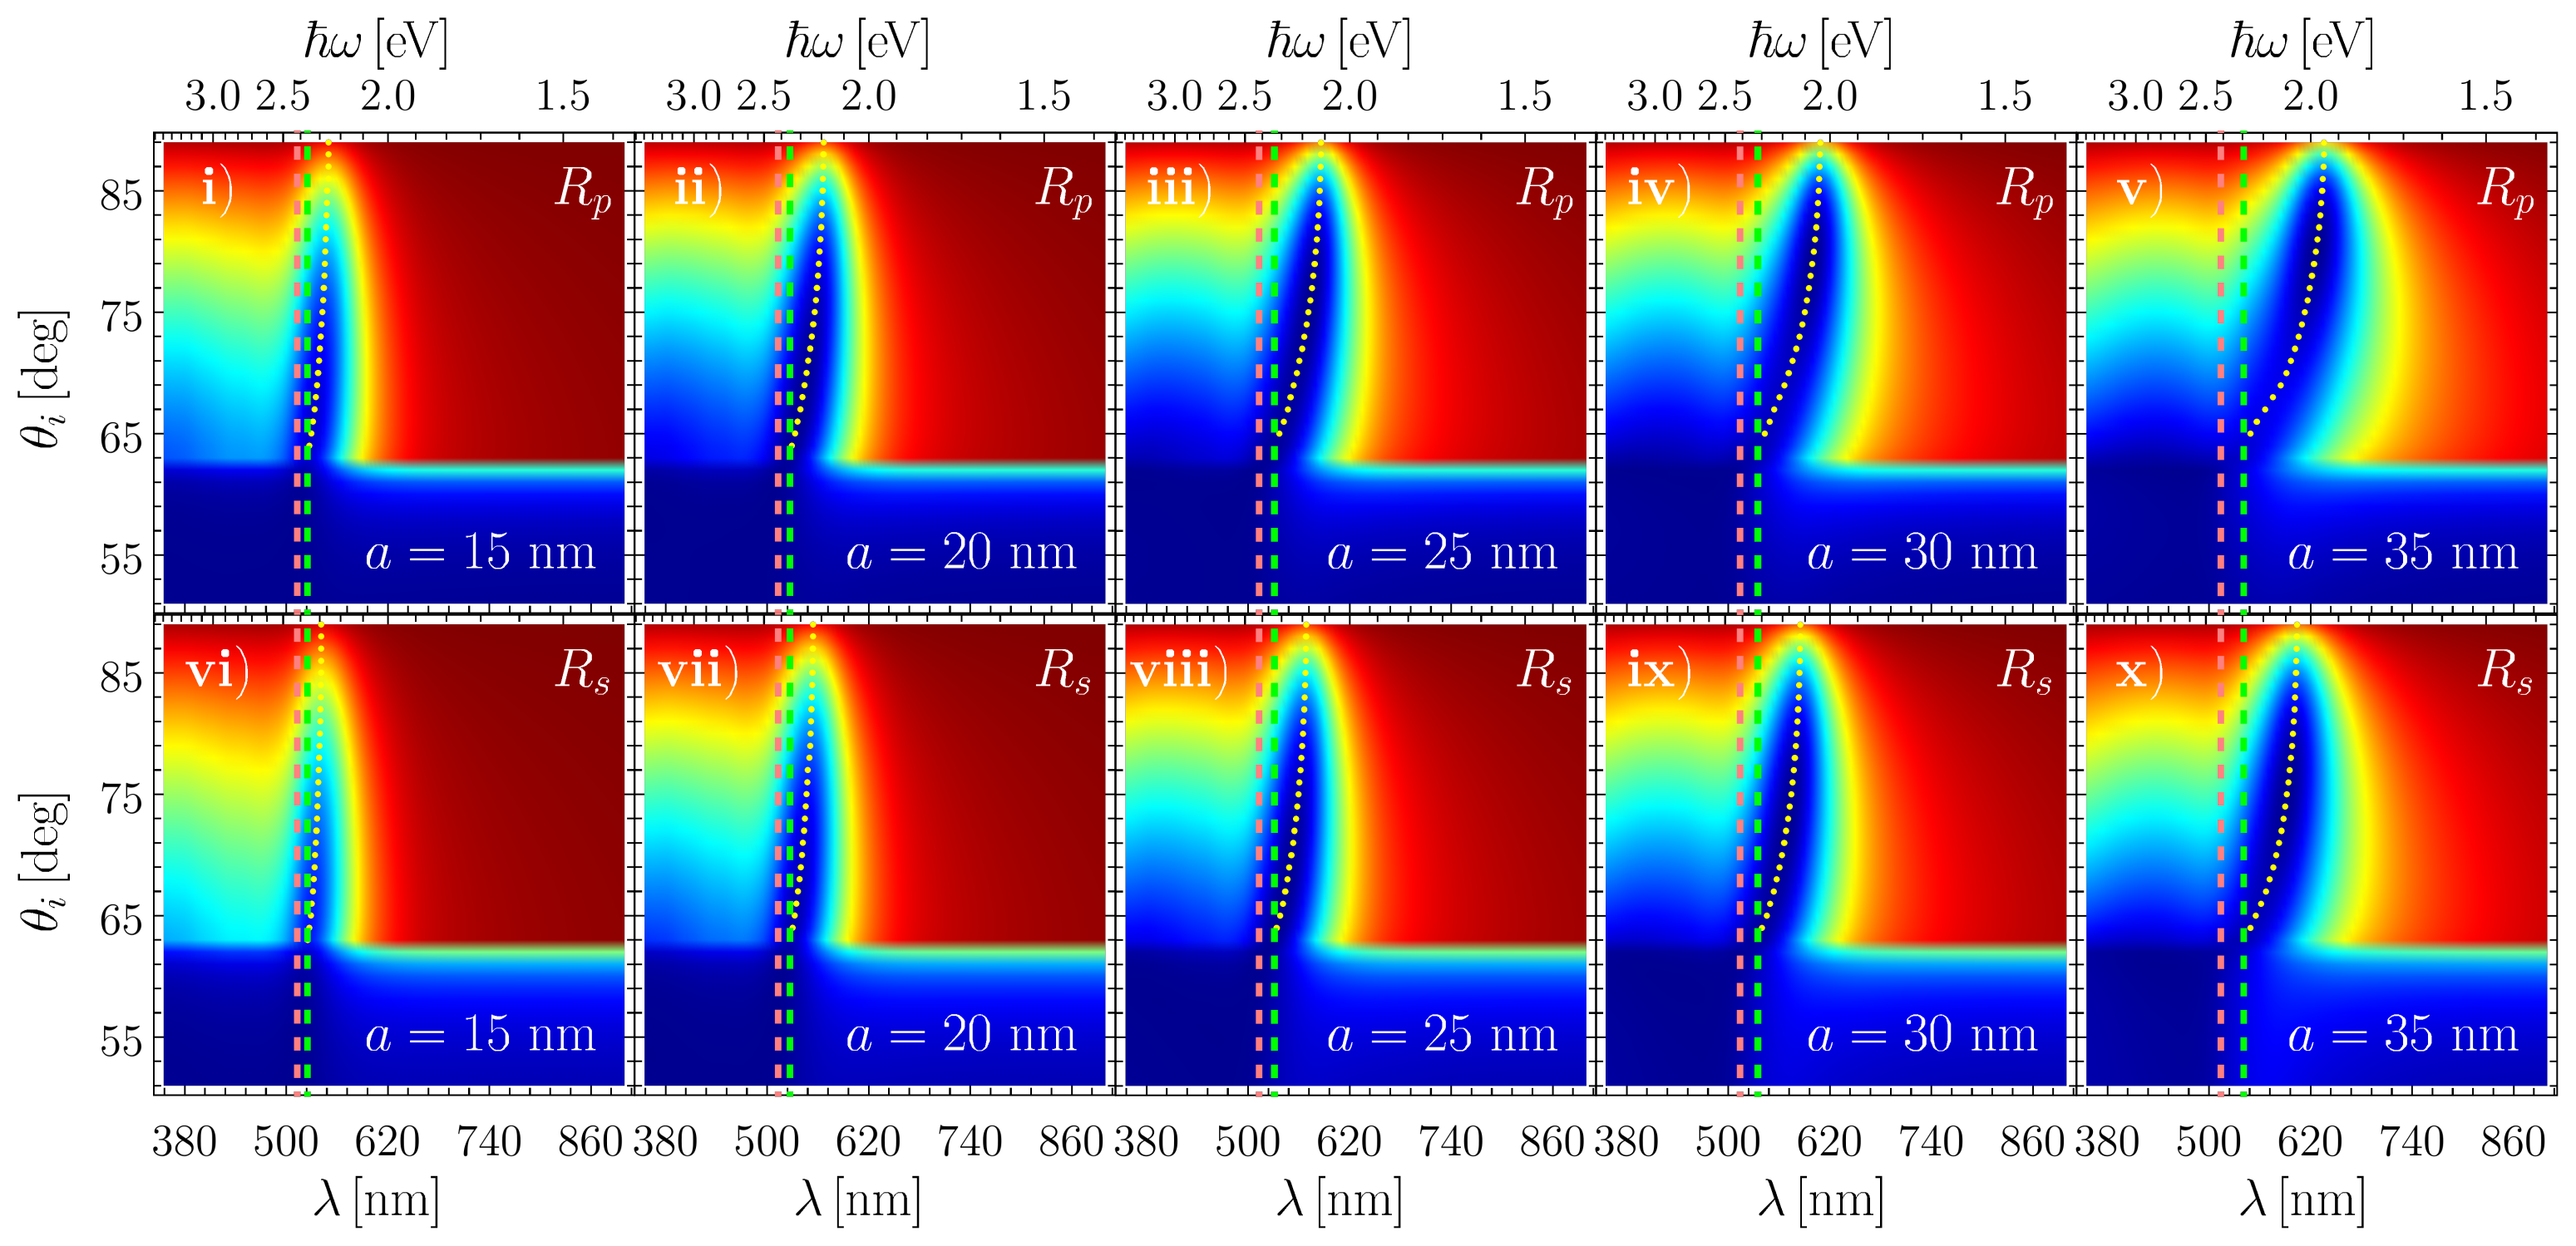
\includegraphics[width = .75\linewidth]{2-Resultados/figs/8-AurVar/0-2D_Grid}%
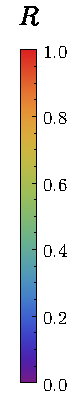
\includegraphics[scale=.85, trim={00 -5 00 00}, clip]{2-Resultados/figs/0-RBar_v}
	\caption{Gráficas de reflectancia de una monocapa en configuración ATR como función del ángulo de incidencia $\theta_i$ y de la longitud de onda $\lambda$ (escala inferior), así como de la energía del haz incidente en unidades de $\hbar\omega$ (escala superior), para una función dieléctrica tipo Drude con $\omega_p=4.3$ eV  y  $\gamma=0. 15$ eV.  Las gráficas   en el renglón superior [$\mathbf{i)-v)}$] muestran los resultados para  polarización \emph{p} y las del renglón inferior  [$\mathbf{vi)-x)}$]  para polarización  \emph{s}, donde se consideró una fracción de cubierta $\Theta = 0.3$ y  NPs de radio  $a$: $3$ nm, $5$ nm, $10$ nm y $20$ nm.  Las líneas verticales punteadas verdes y rosas corresponden a las SP-SPRs dipolar y  cuadrupolar, respectivamente.  Los puntos amarillos corresponden a los mínimos en $R$ para ángulos mayores a $\theta_c\approx 41^\circ$ y longitudes de onda mayores a la SP-SPRs dipolar.
}	\label{fig:R-RVar}	
	\end{figure}	

\begin{figure}[h!]\centering
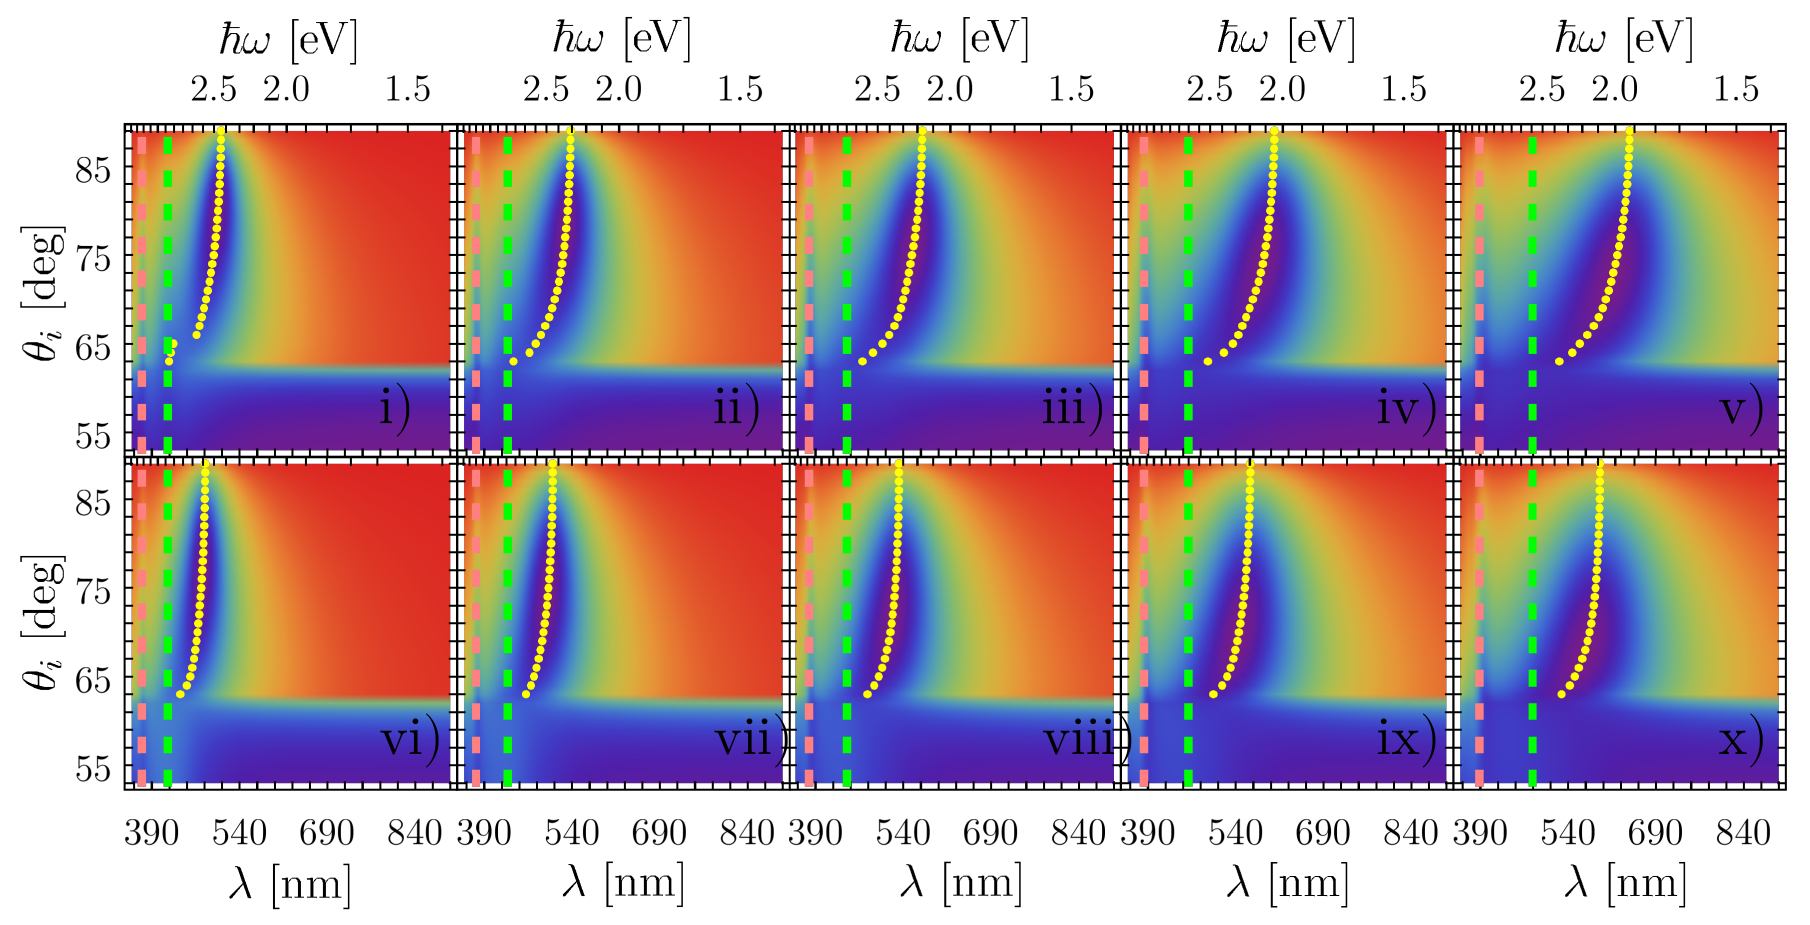
\includegraphics[width = .75\linewidth]{2-Resultados/figs/9-AgrVar/0-2D_Grid}%
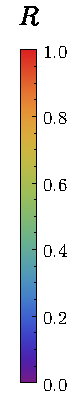
\includegraphics[scale=.85, trim={00 -5 00 00}, clip]{2-Resultados/figs/0-RBar_v}
	\caption{Gráficas de reflectancia de una monocapa en configuración ATR como función del ángulo de incidencia $\theta_i$ y de la longitud de onda $\lambda$ (escala inferior), así como de la energía del haz incidente en unidades de $\hbar\omega$ (escala superior), para una función dieléctrica tipo Drude con $\omega_p=4.3$ eV  y  $\gamma=0. 15$ eV.  Las gráficas   en el renglón superior [$\mathbf{i)-v)}$] muestran los resultados para  polarización \emph{p} y las del renglón inferior  [$\mathbf{vi)-x)}$]  para polarización  \emph{s}, donde se consideró una fracción de cubierta $\Theta = 0.3$ y  NPs de radio  $a$: $3$ nm, $5$ nm, $10$ nm y $20$ nm.  Las líneas verticales punteadas verdes y rosas corresponden a las SP-SPRs dipolar y  cuadrupolar, respectivamente.  Los puntos amarillos corresponden a los mínimos en $R$ para ángulos mayores a $\theta_c\approx 41^\circ$ y longitudes de onda mayores a la SP-SPRs dipolar.
}	\label{fig:R-RVar}	
	\end{figure}	






\begin{figure}[h!]\centering\hspace*{-1.5em}
	\begin{subfigure}{.01\linewidth}\caption{}\label{sfig:R-RVar-cutp}\vspace{4.5cm}\end{subfigure}
	\begin{subfigure}{.45\linewidth}\hspace*{-1.5em}
	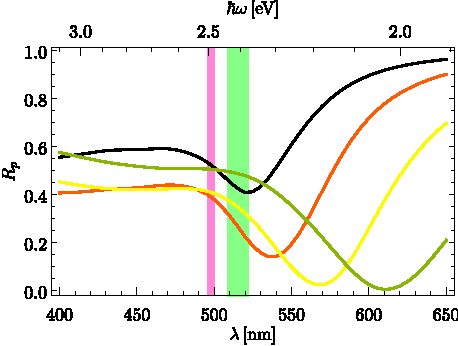
\includegraphics[scale=1]{2-Resultados/figs/8-AurVar/cut_angle_65_p.pdf}\end{subfigure}
	\begin{subfigure}{.01\linewidth}\caption{}\label{sfig:R-RVar-cuts}\vspace{4.5cm}\end{subfigure}\hspace*{-1.em}
	\begin{subfigure}{.45\linewidth}\centering
	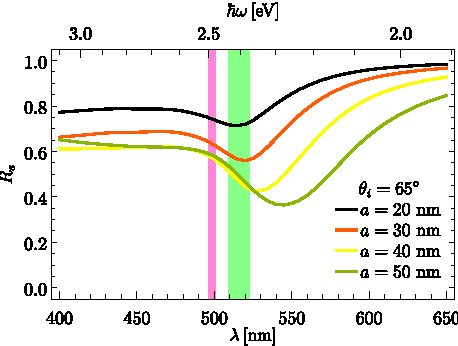
\includegraphics[scale=1 ]{2-Resultados/figs/8-AurVar/cut_angle_65_s.pdf}\end{subfigure}\vspace*{-0em}\\
	\hspace*{-1.5em}
	\begin{subfigure}{.01\linewidth}\caption{}\label{sfig:R-RVar-cutp}\vspace{4.5cm}\end{subfigure}
	\begin{subfigure}{.45\linewidth}\hspace*{-1.5em}
	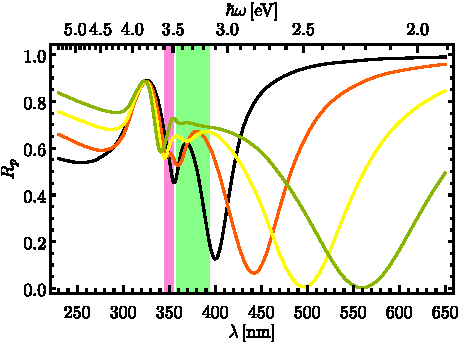
\includegraphics[scale=1]{2-Resultados/figs/9-AgrVar/cut_angle_65_p.pdf}\end{subfigure}
	\begin{subfigure}{.01\linewidth}\caption{}\label{sfig:R-RVar-cuts}\vspace{4.5cm}\end{subfigure}\hspace*{-1.em}
	\begin{subfigure}{.45\linewidth}\centering
	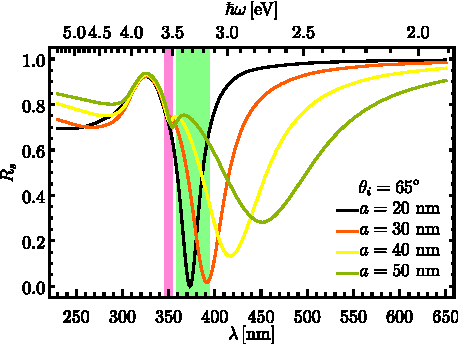
\includegraphics[scale=1 ]{2-Resultados/figs/9-AgrVar/cut_angle_65_s.pdf}\end{subfigure}\vspace*{-.7em}
	\caption{Cortes a $\theta_i = 65^\circ$ de las gráficas de reflectancia de una monocapa en configuración ATR (Fig. \ref{fig:R-RVar}) de NPs esféricas de fracción de cubierta $\Theta = 0.3$ en polarización \textbf{a)} \emph{p} y \textbf{b)} \emph{s} como función de la longitud de onda $\lambda$ (escala inferior) y de la energía $\hbar\omega$ (escala superior). Los parámetros de la función dieléctrica tipo Drude para las NPs son $\omega_p = 4.3$ eV y $\gamma = 0.15$ eV y las fracciones de cubierta consideradas fueron $a$: $3$ nm, $5$ nm, $10$ nm y $20$ nm. La SP-SPR dipolar para los tamaños de partículas utilizadas corresponde la región verde entre $500$ nm y $512$ nm, mientras que la cuadrupolar corresponde a la región rosa entre $456$ nm y $462$ nm.}\label{fig:AuAg-Cuts}
	\end{figure}	








%Finalmente, se emplean las funciones dieléctricas experimentales del oro y la plata \cite{johnson1972constants} para corroborar que el presunto modo colectivo también se presenta en modelos más realistas. Para determinar las SP-SPRs de NPs de oro y plata se presenta en la Fig. \ref{fig:Q-ext} la eficiencia de extinción $Q_{ext}$ (sección transversal de extinción normalizada por la sección transversal geométrica) como función de la longitud de onda $\lambda$ (escala inferior), así como de la energía $\hbar\omega$ (escala superior) del haz incidente. Las SP-SPRs se localizan en los máximos de la $Q_{ext}$ para cada contribución multipolar: la SP-SPR dipolar se localiza en  la longitud de onda $\lambda^{(1)} = 513$ nm para el oro y $368$ nm para la plata, mientas que la SP-SPR cuadrupolar se localiza en $\lambda^{(2)} = 501$ nm para el oro y $348$ nm para la plata. %Todas las excitaciones de origen plasmónico se encunetran entre el modo dipolar $\lambda^{(1)}$ y la SPR de superficie $\lambda^{(\infty)} = \lambda^{(1)}\sqrt{2/3}$, rango de  valores que corresponden a la región gris en la Fig. \ref{fig:Q-ext}. Ya que para el oro la SPR de superficie se localiza en $418$ nm  y para la plata en $300$ nm, cualquier excitación en  la Fig. \ref{sfig:Q-ext-Au} en $\lambda<418$ para el oro no es plasmónica, así como tampoco lo son las excitaciones en la Fig. \ref{sfig:Q-ext-Ag} en $\lambda<300$ nm para la plata.
%
%
%	\begin{figure}[h!]\centering
%	\begin{subfigure}{.01\linewidth}\caption{}\label{sfig:Q-ext-Au}\vspace{3.75cm}\end{subfigure}\hspace*{-.5em}
%	\begin{subfigure}{.45\linewidth}\centering 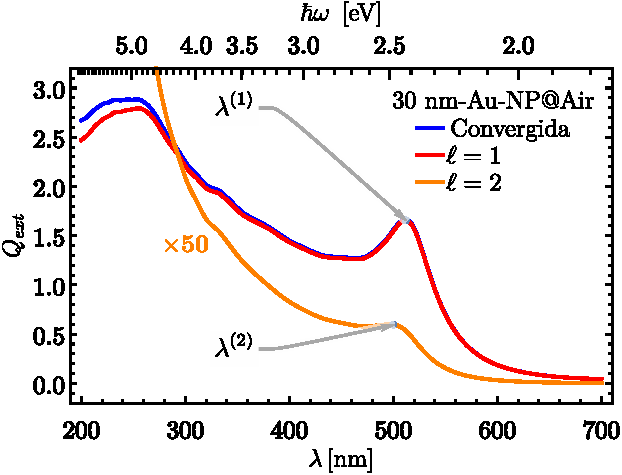
\includegraphics[scale=.75 ]{2-Resultados/figs/5-JCAu/Au_Qexr}\end{subfigure}
%	\begin{subfigure}{.01\linewidth}\caption{}\label{sfig:Q-ext-Ag}\vspace{3.75cm}\end{subfigure}\hspace*{-.5em}
%	\begin{subfigure}{.45\linewidth}\centering 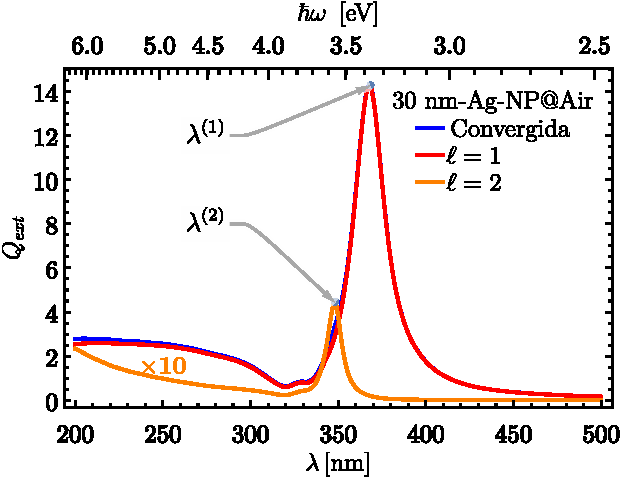
\includegraphics[scale=.75 ]{2-Resultados/figs/6-JCAg/Ag_Qexr.pdf}\end{subfigure}\vspace*{-.5em}
%	\caption{Eficiencia de extinción $Q_{ext}$ de una NP individual de \textbf{a)} oro y de \textbf{b)} plata de radio $a = 30$ nm, inmersa en aire $n_m = 1$ como función de la longitud de onda $\lambda$ (escala inferior), así como de la energía $\hbar\omega$ (escala superior) del haz incidente. En azul se muestra el resultado de $Q_{ext}$ sumando seis contribuciones multipolares (convergida), en rojo se muestra la contribución del modo dipolar ($\ell = 1$) y en naranja la del modo cuadrupolar ($\ell = 2$) con un aumento de $\times 50$ para el oro y $\times 10$ para la plata. La longitud de onda de la SP-SPR dipolar $\lambda^{(1)}$ es $513$ nm para el oro y $368$ nm para la plata; la longitud de onda de la SP-SPR cuadrupolar $\lambda^{(2)}$  es $501$ nm para el oro y $348$ nm para la plata.
%	% La SPR de superfice $\lambda^{(\infty)}$ para el oro se localiza en $418$ nm y para la plata en $300$ nm. La región gris delimita los valores de $\lambda$ entre $\lambda^{(\infty)}$ y $\lambda^{(1)}$, en donde se encuntran todas las excitaciones de origen plasmónico.
%	 }\label{fig:Q-ext}
%	\end{figure}	
%
%
%
%En la Fig. \ref{sfig:JCAu} se calcula la reflectancia de una monocapa de NPs de oro, Fig. \ref{sfig:JCAu}, y plata, Fig. \ref{sfig:JCAg}, con un radio de $a=30$ nm y fracción de llenado $\Theta = 0.3$, inmersas en aire ($n_m = 1$) y soportadas por un sustrato con índice de refracción $n_s = 1.5$, tanto para polarización \emph{p}, gráfica \textbf{i)}, como \emph{s}, gráfica \textbf{ii)}. Las SP-SPRs para ambos materiales corresponden a las líneas punteadas verdes, para el dipolo, y las rosas para el cuadrupolo. Asimismo, todos los mínimos de $R$ corresponden a los puntos amarillos. 
%
%	\begin{figure}[h!]\centering
%	\begin{subfigure}{.01\linewidth}\caption{}\label{sfig:JCAu}\vspace{3cm}\end{subfigure}\hspace*{-1em}
%	\begin{subfigure}{.45\linewidth}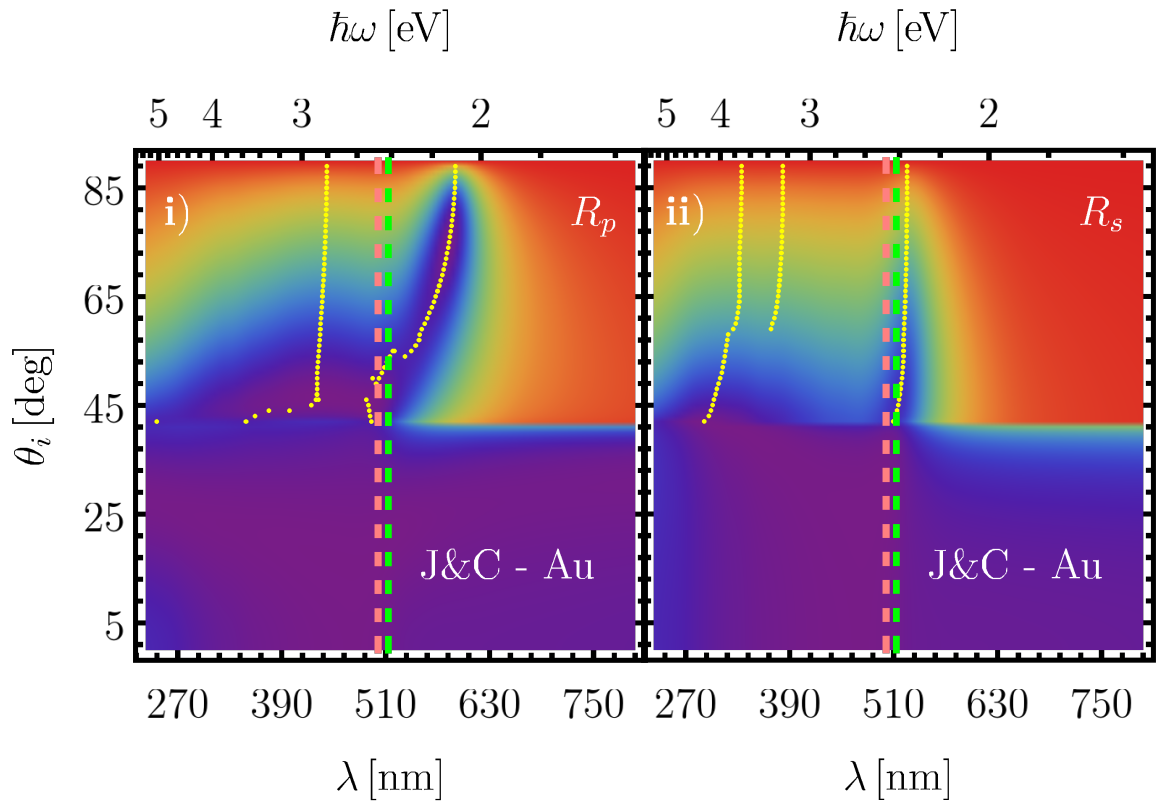
\includegraphics[width = .95\linewidth,]{2-Resultados/figs/5-JCAu/0-2D_Grid.png}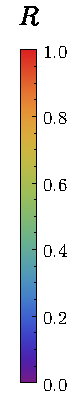
\includegraphics[scale=.6, trim={00 00 00 00}, clip]{2-Resultados/figs/0-RBar_v}
%	\end{subfigure}\hspace*{1em}
%	\begin{subfigure}{.01\linewidth}\caption{}\label{sfig:JCAg}\vspace{3cm}\end{subfigure}\hspace*{-1em}
%	\begin{subfigure}{.45\linewidth}\centering 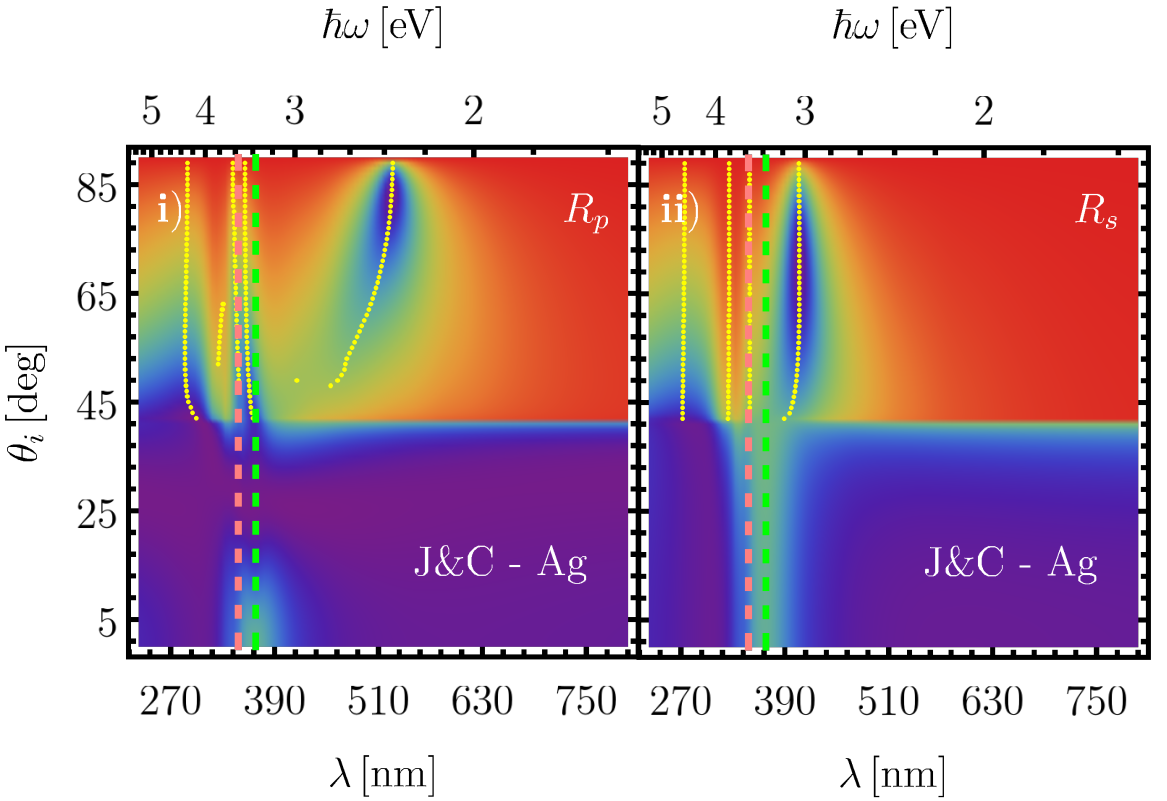
\includegraphics[width = .95\linewidth, trim={00 05 00 00}, clip]{2-Resultados/figs/6-JCAg/0-2D_Grid.png}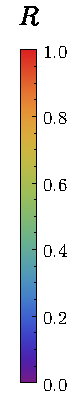
\includegraphics[scale=.6, trim={00 00 00 00}, clip]{2-Resultados/figs/0-RBar_v}\end{subfigure}
%	\caption{Gráficas de reflectancia de una monocapa en configuración ATR ($\Theta = 0. 3$) como función del ángulo de incidencia $\theta_i$ y de la longitud de onda $\lambda$ para NPs de \textbf{a)} Au y \textbf{b)} Ag, calculados con los datos experimentales del índice de refracción tomados de \cite{johnson1972constants}.  Los mínimos en la reflectancia se señalizan mediante los puntos amarillos. }\label{fig:R-JC}
%	\end{figure}	
%
%Para el caso del oro, Fig. \ref{sfig:JCAu},  a ambas polarizaciones son apreciables excitaciones en $\theta_i>\theta_c \approx 41^\circ$ y  $\lambda$ menores a la longitud de onda de la SP-SPR cuadrupolar, así como una excitación a longitudes de onda mayores a la SP-SPR dipolar ($510$ nm). Para ambas polarizaciones, la excitación a las longitudes de onda mayores que la SP-SPR dipolar se comporta como el presunto modo colectivo que se analizó para una monocapa de NPs con una función dieléctrica tipo Drude, es decir, la  excitación en $\lambda>510$ nm coincide con la SP-SPR dipolar en $\theta\approx \theta_c$ y se corre al rojo conforme aumenta el ángulo de incidencia, y la separación entre el valor de la SP-SPR dipolar y la excitación en en $\lambda>510$ nm  es mayor para polarización \emph{p}, gráfica \textbf{i)}, que para polarización \emph{s}, gráfica \textbf{ii)}. Por lo anterior, la presunta respuesta colectiva es apreciable para una monocapa de NPs de oro y se traslapa con la SP-SPR dipolar.
%
%Los resultados de la reflectancia para la monocapa de NPs de plata en la Fig. \ref{sfig:JCAg} presentan, a amabas polarizaciones, una excitación en $\theta_i>\theta_c \approx 41^\circ$ y $\lambda\approx 270$ así como una excitación en la longitud de onda $\lambda \approx 328$ nm y otra que coincide con la SP-SPR cuadrupolar en $\lambda\approx 348$ nm. La respuesta EM de la monocapa presenta una excitación en la longitud de onda cercana a la de la SP-SPR dipolar para polarización \emph{p}, gráfica \textbf{i)}, mientras que en polarización \emph{s}, gráfica \textbf{ii)} no hay una excitación cercana a la longitu de onda de la SP-SPR dipolar. Sin embargo, al igual que para la monocapa de NPs de oro, a longitudes de onda mayores a la SP-SPR dipolar, se observa una excitación que  se corre al rojo conforme aumenta el ángulo de incidencia, así como también aumenta la separación entre ésta y la SP-SPR dipolar para los resultados en polarización \emph{p}, gráfica \textbf{i)}, que en polarización \emph{s}, gráfica \textbf{ii)}. Es decir, el presunto modo colectivo es apreciable también para una monocapa de NPs de plata.
%
%Al analizar la respuesta óptica de una monocapa con NPs modeladas mediante funciones dieléctricas tipo Drude y funciones dieléctricas experimentales, se concluye que el supuesto modo colectivo también es apreciable para modelos de NPs realistas. La excitación del supuesto modo colectivo se observa a energías menores a la excitación dipolar para una partícula individual y se corre al rojo conforme aumenta la fracción de cubierta o el radio de las NPs, es decir, conforme la cantidad de electrones libres presentes en la monocapa crece. Este modo colectivo puede sintonizarse según sean los parámetro empleados para la monocapa, radio de las NPs y fracción de cubierta, además de que puede distinguirse de la SP-SPR dipolar, a pesar del traslape observado entre ellas, dado que la extinción de luz a las longitudes de onda del presunto modo colectivo es mayor que para la SP-SPR dipolar y dado que se corre al rojo conforme la cantidad de electrones libres en la monocapa aumenta.
%
%Para futuros cálculos en la caracterización del supuesto modo colectivo, se buscará la combinación de radios de las NPs y de fracción de cubierta en donde la extinción de luz sea máxima, así como el ancho de banda sea mínimo, para poder emplear el modo colectivo en el biosensado, al igual que la PSLR reportada en \cite{kabashin2009plasmonic} y \cite{danilov2018ultra}. Por tal motivo, se implementará la corrección por tamaño en la función dieléctrica ya que el camino libre medio de los electrones (a $273$ K) es menor a $50$ nm. Asimismo, dado que la PSLR es un modo guiado, se corroborará si el supuesto modo colectivo también es un modo guiado mediante el cálculo de la transmitancia empleando el formalismo del CSM.

